\section{Introducción}\label{sec:introduccion}
\begin{frame}{Simulación regida por tiempo}
    \textbf{Características:}
    \begin{itemize}
        \item N partículas posicionadas horizontalmente una al lado de la otra con resortes entre ellas.
        \item Todas las partículas cuentan con la misma masa.
        \item Las partículas tienen un movimiento principalmente vertical.
        \item La partícula N realiza un movimiento armónico.
    \end{itemize}
\end{frame}

% \begin{frame}{Introducción}
%     \begin{block}{Diagrama:}
%         \begin{figure}
%             \centering
%             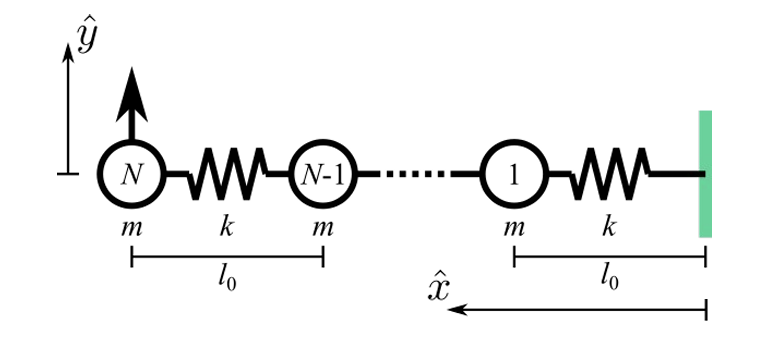
\includegraphics[width=0.8\linewidth]{pic/01-introduccion/diagrama}
%             \label{fig:diagrama}
%         \end{figure}
%     \end{block}
% \end{frame}

%\begin{frame}{Utilizando Verlet en los pasos temporales}
%    \textbf{Fórmulas:}
%
%    \vspace{5pt}
%    \begin{equation*}
%        r_i(t + \Delta{t}) = 2 r_i(t) - r_i(t-\Delta{t}) + \frac{\Delta{t}}{m_i} f_i(t) + O(\Delta{t}^4)
%    \end{equation*}
%
%    \vspace{20pt}
%    \begin{equation*}
%        v_i(t) = \frac{r_i(t+\Delta{t}) + r_i(t-\Delta{t})}{2\Delta{t}} + O(\Delta{t}^3)
%    \end{equation*}
%\end{frame}

\begin{frame}{Modelo}
    \begin{block}{Fuerzas sobre las partículas}
        \begin{equation*}
            \begin{aligned}
                F_i(t+t_0) &= -k\ (y_i - y_{i-1}) - k\ (y_i - y_{i+1})
            \end{aligned}\label{eq:equation-particles-movement}
        \end{equation*}
        Considerando \( y_0 \) como la constante 0
    \end{block}

    \begin{block}{Partícula N}
        Siempre seguirá el movimiento: \begin{equation*} y_{100}=A\ sin(\omega t)\end{equation*}
    \end{block}
\end{frame}


